\documentclass[12pt, a4paper, oneside]{ctexbook}
\usepackage{amsmath, amsthm, amssymb, bm, graphicx, hyperref, mathrsfs}
\usepackage{pifont}
\usepackage{listings}
\usepackage{xcolor}
\usepackage{CJKvert}

\title{{\Huge{\textbf{学习记录-2024}}}}
\author{JiangYiFu}
\date{\today}
\linespread{1.5}
\newtheorem{theorem}{定理}[section]
\newtheorem{definition}[theorem]{定义}
\newtheorem{lemma}[theorem]{引理}
\newtheorem{corollary}[theorem]{推论}
\newtheorem{example}[theorem]{例}
\newtheorem{proposition}[theorem]{命题}

\begin{document}

\maketitle

\pagenumbering{roman}
\setcounter{page}{1}

\begin{center}
    \Huge\textbf{前言}
\end{center}~\


~\\
\begin{flushright}
    \begin{tabular}{c}
        JiangYiFu in USTC\\
        \today
    \end{tabular}
\end{flushright}

\newpage
\pagenumbering{Roman}
\setcounter{page}{1}
\tableofcontents
\newpage
\setcounter{page}{1}
\pagenumbering{arabic}

\chapter{函数极限与连续}


\section{如何求解函数方程}

设函数$f(x)$的定义域为$(0,\infty)$,且满足$2f(x)+x^2f(\frac{1}{x})=\frac{x^2+2x}{\sqrt{1+x^2}}$,则$f(x)=\_\_\_\_$。

key:轮换对称式,高中题目常见

Answer:
\[f(x)=\frac{x}{\sqrt{1+x^2}}\]

\section{反函数}

1.严格单调函数必有反函数。

2.有反函数的不一定是单调函数。

\hspace*{\fill}

求函数$y=f(x)=ln(x+\sqrt{x^2+1})$的反函数$f^{-1}(x)$的表达式及其定义域.

key:注意到代数变形
\[ \frac{1}{x+\sqrt{x^2+1}}=\sqrt{x^2+1}-x\]

Answer:
\[f^{-1}(x)=\frac{e^x-e^{-x}}{2}\]

\section{复合函数的奇偶性}

$f[g(x)]$(内偶则偶,内奇同外)

\hspace*{\fill}

设对任意$x$,$y$,都有$f(x+y)=f(x)+f(y)$,证明:$f(x)$是奇函数.

key:对$x,y$赋值

\hspace*{\fill}

\[f(x)=\frac{2^x-1}{2^x+1},x\in \mathbb{R}\]
计算
\[\int_{-1}^{1}\frac{1}{2^x+1}dx\]

key:注意到$f(x)$是奇函数,且
\[\frac{1}{2^x+1}=\frac{1}{2}\frac{(2^x+1)-(2^x-1)}{2^x+1}\]

\section{三角函数}

\[sec(x)=\frac{1}{cos(x)},csc(x)=\frac{1}{sin(x)}\]

\[1+tan(\alpha)^2=sec(\alpha)^2\]

\section{函数极限定义}

“$\varepsilon - \delta$”语言:
$\lim\limits_{x \to x_0}f(x)=A \iff \forall \varepsilon >0,\exists \delta>0$,当$0<|x-x_0|<\delta$时,有$|f(x)-A|<\varepsilon$.

\hspace*{\fill}

函数极限存在的充要条件:
$\lim\limits_{x \to x_0}f(x)=A \iff \lim\limits_{x \to x_0^-}f(x)=A$且$\lim\limits_{x \to x_0^+}f(x)=A$

\section{极限与有界性}

极限的局部有界性(常用于证明题):如果$\lim\limits_{x \to x_0}f(x)=A$,则存在正常数$M$和$\delta$,使得当$0<|x-x_0|<\delta$时,有$|f(x)|\leq M$.

\hspace*{\fill}

若$y=f(x)$在$[a,b]$上为连续函数,则$f(x)$在$[a,b]$上必定有界.

\hspace*{\fill}

若$f(x)$在$(a,b)$内为连续函数,且$\lim\limits_{x \to a^+}f(x)$与$\lim\limits_{x \to b^-}f(x)$都存在,则$f(x)$在$[a,b]$内必定有界.

\hspace*{\fill}

在下列区间内,函数
\[f(x)=\frac{xsin(x-3)}{(x-1)(x-3)^2}\]
有界的是(\ \ )

A.$(-2,1)$\ \ \ B.$(-1,0)$\ \ \ C.$(1,2)$\ \ \ D.$(2,3)$

key:函数有界问题$\iff$极限存在问题

Answer:B

\hspace*{\fill}

局部保号性(*)

\section{极限:“脱帽法”和“戴帽法”}

$$
    \begin{cases}
	   \lim f > 0 \Rightarrow f > 0 \\
		\lim f < 0 \Rightarrow f < 0 \\
       f \geq 0 \Rightarrow \lim f \geq 0 \\
		f \leq 0 \Rightarrow \lim f \leq 0 

    \end{cases}
$$

\section{无穷小的比阶}

并不是任意两个无穷小都可进行比阶.

\section{极限计算}

极限四则运算规则(*)

\hspace*{\fill}

若$\lim \frac{f(x)}{g(x)}= A$,且$\lim g(x)=0$,则$\lim f(x)=0$.

若$\lim \frac{f(x)}{g(x)}= A \neq 0$,且$\lim f(x)=0$,则$\lim g(x)=0$.

\hspace*{\fill}

设$\lim\limits_{x \to 0} \dfrac{sinx}{e^x - a}(cosx - b)=5$,那么$b=\_\_\_$.

Answer:-4

\section{洛必达法则}

法则一:设

1.当$x\to a$(或$x\to \infty$)时,函数$f(x)$及$F(x)$都趋于零.

2.$f^{'}(x)$及$F^{'}(x)$在点$a$的某去心邻域内(或当$|x|>X$,此时$x$为充分大的正数)存在,且$F^{'}(x) \neq 0$.

3.$\lim\limits_{x \to a} \frac{f^{'}(x)}{F^{'}(x)}$(或$\lim\limits_{x \to \infty} \frac{f^{'}(x)}{F^{'}(x)}$)存在或为无穷大,则

\[\lim\limits_{x \to a} \frac{f(x)}{F(x)}=\lim\limits_{x \to a} \frac{f^{'}(x)}{F^{'}(x)}\]

或

\[\lim\limits_{x \to \infty} \frac{f(x)}{F(x)}=\lim\limits_{x \to \infty} \frac{f^{'}(x)}{F^{'}(x)}\]

注意:这是一个后验逻辑命题

法则二:设

1.当$x\to a$(或$x\to \infty$)时,函数$f(x)$及$F(x)$都趋于无穷大.

2.$f^{'}(x)$及$F^{'}(x)$在点$a$的某去心邻域内(或当$|x|>X$,此时$x$为充分大的正数)存在,且$F^{'}(x) \neq 0$.

3.$\lim\limits_{x \to a} \frac{f^{'}(x)}{F^{'}(x)}$(或$\lim\limits_{x \to \infty} \frac{f^{'}(x)}{F^{'}(x)}$)存在或为无穷大,则

\[\lim\limits_{x \to a} \frac{f(x)}{F(x)}=\lim\limits_{x \to a} \frac{f^{'}(x)}{F^{'}(x)}\]

或

\[\lim\limits_{x \to \infty} \frac{f(x)}{F(x)}=\lim\limits_{x \to \infty} \frac{f^{'}(x)}{F^{'}(x)}\]

\section{泰勒公式}

设$f(x)$在点$x=0$处$n$阶可导,则存在$x=0$的一个邻域,对于该邻域内的任一点$x$,有

\[f(x)=f(0)+f^{'}(0)x+\frac{f^{''}(0)}{2!}x^2 + ... + \frac{f^{(n)}(0)}{n!}x^n + o(x^n).\]

常见结论:

\[sin(x)=x-\frac{x^3}{3!}+o(x^3)\]

\[cos(x)=1-\frac{x^2}{2!}+\frac{x^4}{4!}+o(x^4)\]

\[arcsin(x)=x+\frac{x^3}{3!}+o(x^3)\]

\[tan(x)=x+\frac{x^3}{3}+o(x^3)\]

\[arctan(x)=x-\frac{x^3}{3}+o(x^3)\]

\[ln(1+x)=x-\frac{x^2}{2}+\frac{x^3}{3}+o(x^3)\]

\[e^x=1+x+\frac{x^2}{2!}+\frac{x^3}{3!}+o(x^3)\]

\[(1+x)^{\alpha}=1+\alpha x+\frac{\alpha (\alpha - 1)}{2!}x^2+o(x^2)\]



\section{两个重要极限}

\[\lim\limits_{x \to 0} \frac{sin(x)}{x}=1.\]

\[\lim\limits_{x \to \infty}(1+\frac{1}{x})^x=e.\]


\section{夹逼准则}

如果函数$f(x)$,$g(x)$及$h(x)$满足下列条件:

(1)$h(x)\leq f(x)\leq g(x)$.

(2)$\lim g(x)=A,\lim h(x)=A$.

则$\lim f(x)$存在,且$\lim f(x)=A.$

\section{极限计算例题}

\[\lim\limits_{x \to 0^+}\frac{(1+x)^{\frac{1}{x}}-e}{x}=\_\_\_\]

key:$u^v=e^{vln(u)}$,$e^x-1\~{}  x$

Answer:$-\frac{1}{2}e$

注意:记忆$f(x)=(1+x)^{\frac{1}{x}}$和$f(x)=(1+\frac{1}{x})^{x}$的函数图像

\hspace*{\fill}

设函数\[f(x)=\lim\limits_{n \to \infty} \frac{x^2 + nx(1-x)sin^2\pi x}{1+nsin^2\pi x}\]

则$f(x)=\_\_\_.$

key:$n\to \infty$专指$n\to +\infty$,将x视作常数

Answer:$$f(x)=\begin{cases}x^2,\quad &x=k\\x(1-x),\quad &x\neq k\end{cases}(k\in Z)$$

\hspace*{\fill}

求极限\[\lim\limits_{x \to 1^-}ln(x)ln(1-x).\]

key:等价代换后换元,转换为

\[\lim\limits_{x \to 0^+}x^{\alpha}ln(x)=\lim\limits_{x \to 0^+} \frac{ln(x)}{x^{-\alpha}}\]

\hspace*{\fill}

求极限
\[\lim\limits_{x \to +\infty}[x^2(e^{\frac{1}{x}}-1)-x].\]

key:代数变形,减法变乘法,换元

Answer:$\frac{1}{2}$

\hspace*{\fill}

求极限
\[\lim\limits_{x \to +\infty}(x+\sqrt{1+x^2})^{\frac{1}{x}}\]

key:幂指函数

Answer:1

\section{函数的连续和间断}

连续点的定义:

设函数$f(x)$在点$x_0$的某一邻域内有定义,且有$\lim\limits_{x \to x_0}f(x)=f(x_0)$,则称函数$f(x)$在点$x_0$处连续.

考察本质是极限的计算.

\hspace*{\fill}

连续判定:

\[\lim\limits_{x \to x_0^+}f(x)=\lim\limits_{x \to x_0^-}f(x)=f(x_0) \iff f(x)\ is\ coiled\ in\ x_0\]

\hspace*{\fill}

连续性四则运算法则(*)

\hspace*{\fill}

间断点的定义和分类:

1.可去间断点(*)

2.跳跃间断点(*)

3.无穷间断点(*)

4.振荡间断点(*)

\chapter{数列极限}

求极限

\[\lim\limits_{n \to \infty}(\frac{1}{1\cdot2}+\frac{1}{2\cdot3}+\cdot \cdot \cdot +\frac{1}{n\cdot (n+1)})^n\]

key:$1^{\infty}$形式,考虑$\lim u^v=\lim e^{v ln(u-1)}$

Answer:$e^{-1}$

\section{数列极限定义}

设$\{x_n\}$为一数列,若存在常数$a$,对于任意的$\epsilon >0$,总存在正整数$N$,使得当$n>N$时,$|x_n-a|<\epsilon$恒成立,则称常数$a$是数列$\{x_n\}$的极限,或者称数列$\{x_n\}$收敛于$a$.

\section{数据收敛与其子列收敛}

若数列{$a_n$}收敛,则其任何子列{$a_{n_k}$}也收敛,且\[\lim\limits_{k \to \infty}a_{n_k}=\lim\limits_{n \to \infty}a_n\].

通过该结论判断数列发散

1.找到一个发散子列

2.找到两个收敛子列,但它们收敛到不同极限。

\hspace*{\fill}

\section{收敛数列的性质}

唯一性(*)

有界性(*)

保号性(*)

\hspace*{\fill}

已知$a_n=1-\frac{(-1)^n}{n}$,则{$a_n$}是否有最大值和最小值?

key:保号性

Answer:有,有


\section{极限四则运算规则}

四则运算规则可以推广至有限个数列情形.

\hspace*{\fill}


\section{海涅定理(归结原则)}

\[\lim\limits_{x \to a}f(x)=L \iff \forall\{a_n\},if\ \lim\limits_{n \to \infty}a_n=a,have\ \lim\limits_{n \to \infty}f(a_n)=L\]

海涅定理是联系数列极限和函数极限的桥梁.

\hspace*{\fill}

当$x \to 0$时,$\frac{1}{x}sin\frac{1}{x}$是\_\_\_?

key:取$x_n=\frac{1}{n\pi}$和$x^{'}_n=\frac{1}{(2n+\frac{1}{2})\pi}$

Answer:无界量,但不是无穷大

\hspace*{\fill}


求\[\lim\limits_{n \to \infty}\sqrt[n]{(cos\frac{1}{\sqrt{n}})^{n^2}}\].

key:通过海涅定理将其转化为函数极限

Answer:$e^{-\frac{1}{2}}$

\hspace*{\fill}


\section{夹逼准则}

假设有三个数列 ${a_n}$,${b_n}$ 和 ${c_n}$,满足以下条件:

1.对于所有的 $n$,有 $a_n \leq b_n \leq c_n$

2.当 $n$ 趋向于正无穷时,${a_n}$ 和 ${c_n}$ 的极限都是 $L$,即 $\lim\limits_{n \to \infty} a_n = \lim\limits_{n \to \infty} c_n = L$

那么 ${b_n}$ 的极限也存在,并且 $\lim\limits_{n \to \infty} b_n = L$

\hspace*{\fill}

\[\lim\limits_{n \to \infty}(\frac{1}{n^2+n+1}+\frac{2}{n^2+n+2}+...+\frac{n}{n^2+n+n})=\_\_\_.\]

key:放缩

Answer:$\frac{1}{2}$

\hspace*{\fill}

求极限\[\lim\limits_{n \to \infty}\sqrt[n]{a_1^n+a_2^n+...+a_m^n}\]
其中$a_i>0$.

key:$a=max\{a_1,a_2,...,a_m\}$

Answer:1

\hspace*{\fill}

类似的题目(利用极限定义函数):\[\lim\limits_{n \to \infty}\sqrt[n]{\sin(x)^n+\cos(x)^n}\]

\hspace*{\fill}

放缩技巧:
1.无穷项相加
\[n\cdot u_{min}\leq u_1+u_2+...+u_n \leq n\cdot u_{max}\]

2.有限项相加
\[u_{max}\leq u_1+u_2+...+u_n \leq n\cdot u_{max} \]


\hspace*{\fill}

设$0<a_n<\dfrac{\pi}{2}$,$0<b_n<\dfrac{\pi}{2}$,$\cos(a_n)-a_n=\cos(b_n)$,且$\lim\limits_{n \to \infty}b_n=0$,求$\lim\limits_{n \to \infty}a_n$,$\lim\limits_{n \to \infty}{\dfrac{a_n}{b_n^2}}$.

\hspace*{\fill}

key:1.分清约束式,关系式,定义式。2.考虑对关系式进行一些恒等变形。

\[\cos a_n -\cos b_n = a_n >0\]


3.联想一些经典形式。\[1-\cos x \sim \dfrac{1}{2}x^2\]

Answer:$\lim\limits_{n \to \infty}a_n=0$,$\lim\limits_{n \to \infty}{\dfrac{a_n}{b_n^2}}=\dfrac{1}{2}$


\hspace*{\fill}

设$a_n>0$,$\lim\limits_{n \to \infty}b_n = 0$,且$e^{a_n}+a_n=e^{b_n}$,$n=1,2,...$,求$\lim\limits_{n \to \infty}a_n$.

key:恒等变换得到$e^{a_n}-e^{b_n}=-a_n<0$

Answer:0

\section{单调有界准则}

单调有界数列必有极限,即若数列{$x_n$}单调增加(减少)且有上界(下界),则$\lim\limits_{n \to \infty}x_n$存在.

\hspace*{\fill}

如何证明数列单调(*)

\hspace*{\fill}

设$0<x_1<3$,$x_{n+1}=\sqrt{x_n(3-x_n)}(n=1,2,...)$,证明数列{$x_n$}的极限存在,并求此极限.

key:作差判断单调性

\hspace*{\fill}

(1)证明方程$x=\cos x$在$(0,\dfrac{\pi}{3})$内有唯一实根$a$;

(2)设$-1\leq x_1 \leq 1$,定义$x_{n+1}=\cos x_n,n=1,2,...$,证明$\lim\limits_{n \to \infty}x_n$存在,且极限值就是(1)中的$a$.

\hspace*{\fill}


设{$x_n$}满足$x_{n+1}^2=2^{x_n},x_1=\sqrt{2},n=1,2,...$,证明{$x_n$}收敛,并求$\lim\limits_{n \to \infty}x_n$.

key:$x_{n+1}=f(x_n)$,分析单调性

Answer:$\lim\limits_{n \to \infty}x_n=2$

\hspace*{\fill}



\chapter{一元函数微分学的概念}

\section{导数定义}

导数定义(*)

\[f'(x)=\lim\limits_{\Delta x \to 0}\dfrac{\Delta y}{\Delta x}=\lim\limits_{\Delta x \to 0}\dfrac{f(x_0+\Delta x)-f(x_0)}{\Delta x} \]

\hspace*{\fill}

下面这三种说法是等价的:

(1)$y=f(x)$在点$x_0$处可导

(2)$y=f(x)$在点$x_0$处导数存在

(3)$f'(x)=A$($A$为有限数)


\hspace*{\fill}


函数在一点可导的充要条件(*)

$f'(x_0)$存在$\iff$其左导数$f'_{-}(x_0)$与右导数$f'_{+}(x_0)$都存在且相等

\hspace*{\fill}

若$f(x)$是可导的偶函数,则$f'(x)$是奇函数.

若$f(x)$是可导的奇函数,则$f'(x)$是偶函数.

\hspace*{\fill}

设$f(x)=\ln (1-x) -\ln(1+x),-1<x<1$.则$f''(x)=\_\_\_$.

key:$f(x)$是奇函数

Answer:0

\hspace*{\fill}


设$f(x)=\dfrac{1}{2^x+1},x\in R$.则$f^{(4)}(0)=\_\_\_$

\hspace*{\fill}

key:$f(x)=\dfrac{1}{2^x+1}-\dfrac{1}{2}$是奇函数.

Answer:0

\hspace*{\fill}

若$f(x)$是可导的周期为$T$的周期函数,则$f'(x)$也是以$T$为周期的周期函数.


\section{导数例题}

设$f(x)$在$x=0$的某邻域内有定义,并且$|f(x)|\leq 1-\cos x$,则$f(x)$在$x=0$处\_\_\_.

key:夹逼准则,导数定义式

Answer:可导且$f'(0)=0$

\hspace*{\fill}

设函数$f(x)=(e^x-1)(e^{2x}-2)...(e^{nx}-n),n \in N$,则$f'(0)=\_\_\_$.

key:取$g(x)=(e^{2x}-2)...(e^{nx}-n)$.

Answer:$(-1)^{n-1}(n-1)!$

\hspace*{\fill}


设$f(x)$在$x=a$处连续,$F(x)=f(x)|x-a|$,则$f(a)=0$是$F(x)$在$x=a$处可导的\_\_\_.

key:作为结论记忆,证明通过定义

Answer:充要条件

\hspace*{\fill}

设$f(x)$在$x=0$处可导,$f(\dfrac{1}{n})=\dfrac{2}{n},n=1,2,...$,则$f'(0)=\_\_\_$.

key:特殊化思想,归结原则计算$f(0)$,对导数定义式继续归结原则.

归结原则$\iff$函数极限存在时通过数列极限计算.

Answer:2

\hspace*{\fill}

设$f(x)=\dfrac{1}{n^2},\dfrac{1}{(n+1)^2}< x \leq \dfrac{1}{n^2},n=1,2,...$.$f(0)=0$.则$f'_{+}(0)=\_\_\_$.

key:本质是极限计算问题,考虑夹逼准则.

Answer:1

\hspace*{\fill}

设可导函数$f(x)>0$,则$\lim\limits_{n \to \infty}n\ln \dfrac{f(\dfrac{1}{n})}{f(0)}=\_\_\_$.

\hspace*{\fill}

key:恒等变换,归结原则(注意其使用条件)

Answer:$\dfrac{f'(0)}{f(0)}$

\hspace*{\fill}

设函数$f(x)$可导,$|f(x)|$在$x=0$处不可导,则\_\_\_.

(学会对于带绝对值的函数导数处理方法)

key:$|f(x)|'=(\sqrt{f^2(x)})'$,可导的极限定义

Answer:$f(0)=0,f'(0)\neq 0$

\hspace*{\fill}

\section{导数的几何意义}


设曲线$y=f(x)=x^n$在点$(1,1)$处的切线与$x$轴的交点为$(\zeta_n,0)$,则$\lim\limits_{n \to \infty}f(\zeta_n)=\_\_\_.$

key:切线定义

Answer:$e^{-1}$

\hspace*{\fill}

设函数$f(x)$连续,$\lim\limits_{x \to 1}\dfrac{f(x)-1}{\ln x}=2.$则曲线$y=f(x)$在$x=1$处的切线方程为\_\_\_.

key:$y-f(1)=f'(1)(x-1)$

Answer:$y=2x-1$

\hspace*{\fill}


\section{高阶导数}

$n$阶导数定义式(*)

\hspace*{\fill}

(1)如果$f(x)$在点$x_0$处有二阶导数,则$f(x)$在$x_0$的某个邻域内有一阶导数且$f'(x)$在$x_0$处连续.

(2)如果$f(x)$在点$x_0$处有$n$阶导数,则$f(x)$在$x_0$的某个邻域内有$1\sim n-1$阶导数.


\section{微分的概念}

微分的概念(*)

\hspace*{\fill}

可微的判别:

(1)写增量$\Delta y=f(x_0+\Delta x)-f(x_0)$.

(2)写线性增量$A\Delta x=f'(x_0)\Delta x$.

(3)作极限$\lim\limits_{\Delta x \to 0}\dfrac{\Delta y-A\Delta x}{\Delta x}$.

如果极限等于0,则$y=f(x)$在$x_0$处可微,否则不可微.

\hspace*{\fill}

$f(x)$在点$x_0$处可微$\iff$$f(x)$在点$x_0$处可导

\hspace*{\fill}

可微的几何意义$\iff$若$f(x)$在点$x_0$处可微,则在点$(x_0,y_0)$附近可以用切线段近似代替曲线段

\hspace*{\fill}

设函数$f(u)$可导,且$y=f(x^2)$,当自变量$x$在$x=-1$处取得增量$\Delta x= -0.1$时,相应的函数增量$\Delta y$的线性主部为0.1,则$f'(1)=\_\_\_.$

key:$y=f[g(x)]$

Answer:$\dfrac{1}{2}$

\hspace*{\fill}



\chapter{一元函数微分学的计算}

\section{基本求导公式}

\[(x^{\alpha})'=\alpha x^{\alpha -1}\]

\[(a^x)'=a^x\ln a\]

\[(\log_a x)'=\dfrac{1}{x\ln a}\]

\[(\ln |x|)'=\dfrac{1}{x}\]

\[(\sin x)'=\cos x\]

\[(\cos x)'=-\sin x\]

\[(\arcsin x)'=\dfrac{1}{\sqrt{1-x^2}}\]

\[(\arccos x)'=-\dfrac{1}{\sqrt{1-x^2}}\]

\[(\tan x)'=\sec ^2 x\]

\[(\arctan x)'=\dfrac{1}{1+x^2}\]

\[[\ln(x+\sqrt{x^2+1})]'=\dfrac{1}{\sqrt{x^2+1}}\]

\[[\ln(x+\sqrt{x^2-1})]'=\dfrac{1}{\sqrt{x^2-1}}\]


\section{四则运算}

函数导数四则运算法则(*)

\hspace*{\fill}


设$f(x)=\Pi_{n=1}^{100}(\tan \dfrac{\pi x^n}{4}-n)$,则$f'(1)=\_\_\_.$

key:令$g(x)=(\tan \dfrac{\pi x^2}{4}-2)...(\tan \dfrac{\pi x^n}{4}-n)$.

Answer:$-\dfrac{\pi}{2}99!$

\hspace*{\fill}



\section{复合函数的导数与微分形式不变性}

\[\{f[g(x)]\}'=f'[g(x)]g'(x)\]

微分形式的不变性:$d\{f[g(x)]\}=f'[g(x)]g'(x)dx=f'[g(x)]d[g(x)]$.也就是说,无论$u$是中间变量还是自变量,$dy=f'(u)du$都成立.

\hspace*{\fill}

注意:$\{f[g(x)]\}'=\dfrac{d\{f[g(x)]\}}{dx}$,$f'[g(x)]=\dfrac{d\{f[g(x)]\}}{dg(x)}$

\hspace*{\fill}

设$y=e^{\sin(\ln x)}$,求$dy$和$\dfrac{dy}{dx}$



\section{分段函数的导数}

(1)在分段点$x_0$处用导数定义求导

(2)非分段点用导数公式

\hspace*{\fill}


设函数$y=|xe^{-x}|$,求$y''(x)$.

key:带绝对值的函数是常考点,需要多多注意

Answer:$y''(x)=\begin{cases}
(x-2)e^{-x} & x > 0 \\
(2-x)e^{-x} & x < 0 \\
\end{cases}
$

\hspace*{\fill}


\section{反函数的导数}

设$y=f(x)$为单调可导函数,且$f'(x)\neq 0$,则存在反函数$x=\varphi (y)$,且$\dfrac{dx}{dy}=\dfrac{1}{\dfrac{dy}{dx}}$,即$\varphi '(y)=\dfrac{1}{f'(x)}$.

\hspace*{\fill}

反函数的二阶导数(*)

注意自己推导:$y''_{xx}=-\dfrac{x''_{yy}}{(x'_y)^3},x''_{yy}=-\dfrac{y''_{xx}}{(y'_{x})^3}$


\section{隐函数求导法}


隐函数求导法具体过程(*)


\section{参数方程所确定的函数的导数}

参数方程所确定的函数的导数求导过程(*)

\hspace*{\fill}

由参数方程确定的函数的二阶导数(*)

\hspace*{\fill}

设函数$y=y(x)$由$\begin{cases}
x = \arctan t \\
2y-ty^2+e^t=5 \\
\end{cases}
$所确定,则$\dfrac{dy}{dx}=\_\_\_.$

Answer:$\dfrac{y^2-e^t}{2(1-ty)}(1+t^2)$

\hspace*{\fill}


\section{对数求导法}

对于多项相乘or相除or开方or乘方的式子,一般先取对数再求导.

对数求导法的具体过程(*)

\hspace*{\fill}

设函数$y=y(x)$由方程$xe^{f(y)}=e^y\ln 2$确定,其中$f$具有二阶导数,且$f'\neq 1$,则$\dfrac{d^2 y}{d x^2}=\_\_\_.$

key:取对数

Answer:$\dfrac{f''(y)-[1-f'(y)]^2}{x^2[1-f'(y)]^3}$

\hspace*{\fill}


\section{幂指函数求导法}

\[u(x)^{v(x)}=e^{v(x)\ln u(x)}\]

\hspace*{\fill}

求函数$y=x^x(x>0)$的导数.

Answer:$x^x (\ln x + 1)$

\hspace*{\fill}

\section{高阶导数}

求高阶导数主要有三种方法:

(1)归纳法.

逐次求导,探索规律,得出通式.

(2)莱布尼茨公式.

\[(uv)^{(n)}=\sum_{k=0}^{n} \binom{n}{k}u^{(n-k)}v^{k}\]

(3)泰勒展开式.

通过记忆一些常见的展开式,来反推$n$阶导数.

\hspace*{\fill}

设$y=\dfrac{1-x}{1+x}$,则$y^{(n)}(0)=\_\_\_.$

key:转化为几种常见形式.

Answer:$(-1)^n 2 \cdot n!$

\hspace*{\fill}

设$f(x)=xe^x$,则$f^{(n)}(x)=\_\_\_.$

key:莱布尼茨公式.

Answer:$(n+x)e^x$

\hspace*{\fill}

设$f(x)=x^2 \ln (1-x)$,则当$n \geqslant 3$时,$f^{(n)}(0)=\_\_\_.$

key:泰勒展开式.

Answer:$-\dfrac{n!}{n-2}$

\hspace*{\fill}

设$f(x)=x^2 2^x$,则当$n \geqslant 1$,$f^{(n)}(0)=\_\_\_.$

key:莱布尼茨公式.

Answer:$n(n-1)(\ln 2)^{n-2}$

\hspace*{\fill}

\chapter{一元微分学的应用---几何应用}

\section{极值的定义}

对于函数$f(x)$,若存在点$x_0$的某个邻域,使得在该邻域内任意一点$x$,均有\[f(x)\leq f(x_0) (f(x)\geqslant f(x_0))\]则称点$x_0$为$f(x)$的极大值点(极小值点),$f(x_0)$为$f(x)$的极大值(或极小值).

\hspace*{\fill}

\textbf{间断点可以是极值点吗?Yes!}

\section{单调性与极值的判别}

单调性的判别:

设函数$y=f(x)$在$[a,b]$上连续,在$(a,b)$内可导.

1.如果在$(a,b)$内$f'(x)\geq 0$,且等号仅在有限个点处成立,那么函数$y=f(x)$在$[a,b]$上严格单调增加.

2.如果在$(a,b)$内$f'(x)\neq 0$,且等号仅在有限个点处成立,那么函数$y=f(x)$在$[a,b]$上严格单调减小.

\hspace*{\fill}


判别极值的第一充分条件(*)(导数变号)

\hspace*{\fill}

判别极值的第二充分条件(*)(二阶导数)

\hspace*{\fill}

判别极值的第三充分条件(*)($n$阶导数)

\hspace*{\fill}

设函数$f(x)$可导,且$f(x)f'(x)>0$,则\_\_\_.

key:联想到$(f^2(x))'$

Answer:$|f(1)|>|f(-1)|$

\hspace*{\fill}

$f''(x_0)<0$(在$f'(x_0)=0$条件下)是$f(x)$在$x_0$处取得极大值的充分不必要条件.

\hspace*{\fill}


\section{凹凸性和拐点的概念}

凹凸性的定义(*)

凹函数:

\[f(\dfrac{x_1+x_2}{2})<\dfrac{f(x_1)+f(x_2)}{2}.\]


设$f(x)$在$[a,b]$上连续,在$(a,b)$内可导,若对$(a,b)$内的任意$x$及$x_0$($x\neq x_0$),均有\[f(x_0)+f'(x_0)(x-x_0)<f(x)\]

\hspace*{\fill}

拐点的定义:

连续曲线的凹弧与凸弧的分界点称为该曲线的拐点.

\section{凹凸性与拐点的判别}

判别凹凸性(*)(二阶导数符号)

\hspace*{\fill}

拐点$\Rightarrow$$f''(x_0)=0+f''(x_0)$不存在

\hspace*{\fill}

判别拐点的第一充分条件(*)(连续+二阶导数变号)

判别拐点的第二充分条件(*)(三阶导数不为0)

判别拐点的第三充分条件(*)($n$阶导数)

\hspace*{\fill}


\section{极值点与拐点的重要结论}

\textbf{结论1:}曲线的可导点不可同时为极值点和拐点,曲线的不可导点可同时为极值点和拐点.

\textbf{结论2:}设多项式函数$f(x)=(x-a)^n g(x)(n>1)$,且$g(a)\neq 0,$则当$n$为偶数时,$x=a$是$f(x)$的极值点;当$n$为奇数时,点$(a,0)$是曲线$f(x)$的拐点;


\section{渐近线}

铅直渐近线定义(*)

水平渐近线定义(*)

斜渐近线定义(*)

寻找渐近线的顺序(*)

\hspace*{\fill}

求曲线$y=\dfrac{1}{x}+\ln(1+e^x)$.

\hspace*{\fill}

key:思考方向是从三类渐近线各自入手考虑

1.无定义点$x=0$  

2.求$\lim\limits_{x \to +\infty}y$,$\lim\limits_{x \to -\infty}y$

3.求$\lim\limits_{x \to +\infty}\dfrac{y}{x}$,$\lim\limits_{x \to +\infty}y-ax$

Answer:$x=0$,$y=x$,$y=0$

\hspace*{\fill}


\section{最值或取值范围}

最值的定义(*)

最值点和极值点的关系:

如果$f(x)$在区间$I$上有最值点$x_0$,并且此最值点$x_0$不是区间$I$的端点而是$I$内部的点,那么此$x_0$必是$f(x)$的一个极值点.

\hspace*{\fill}

求区间$(a,b)$内连续函数$f(x)$的最值或取值范围.

\hspace*{\fill}

\section{作函数图像}

作图的一般步骤:

1.确定定义域,考察函数是否有奇偶性,周期性,并用好图像变换

2.用导数工具(一阶导数确定函数的单调区间和极值点;二阶导数确定曲线的凹凸区间和拐点)

3.考查渐近线

4.作出函数图像

\hspace*{\fill}

常用平面图形(见目录)

\hspace*{\fill}

画出$y=x^x(x>0)$的图像.

\hspace*{\fill}

画出$y=\dfrac{e^x}{x}$的图像.

\hspace*{\fill}

画出$r=\sin ^ 2 \theta (0\leq \theta \leq \pi)$在直角坐标系和极坐标系下的图像.

\hspace*{\fill}


\section{曲率及曲率半径}

设$y(x)$二阶可导,则曲线$y=y(x)$在点$(x,y(x))$处的曲率公式为\[k=\dfrac{|y''|}{[1+(y')^2]^{\dfrac{3}{2}}}\]曲率半径的计算公式为\[R=\dfrac{1}{k}=\dfrac{[1+(y')^2]^{\dfrac{3}{2}}}{|y''|}\]

\chapter{一元函数微分学的应用---中值定理and微分等式and微分不等式}

\section{中值定理}

\begin{theorem}
  (有界与最值定理) 设$f(x)$在$[a,b]$上连续,则$m\leq f(x) \leq M$,其中$m,M$分别为$f(x)$在$[a,b]$上的最小值与最大值.
\end{theorem}



\chapter{行列式基础知识}












\chapter{CS229: Machine Learning---Supervised learning}

\textbf{Supervised learning(监督学习)}

  \begin{figure}[h]
		\centering 
		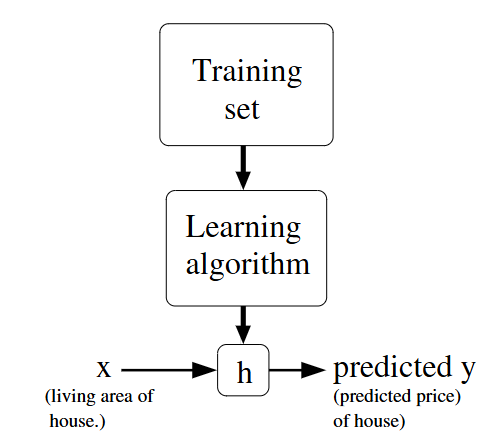
\includegraphics[width=0.45\textwidth]{images18.png} 
	\end{figure}

简单来说就是给定一个数据集,我们使用机器学习算法学习得到一个函数$h$,使得它是一个对于$y$值的良好预测器.

\section{Linear regression}

对于线性回归问题,我们的函数假设为\[h(x)=\sum_{i=0}^{d} \theta_i x_i=\theta^{T}x\]同时定义成本函数\[J(\theta)=\dfrac{1}{2}\sum_{i=1}^{n}(h_{\theta}(x^{(i)})-y^{(i)})^2\]我们想要选择$\theta$使得$J(\theta)$最小化,故而考虑梯度下降算法\[\theta_{j}:=\theta_{j}-\alpha \dfrac{\partial}{\partial \theta_{j}}J(\theta)\]经过计算我们可得\[\dfrac{\partial}{\partial \theta_{j}}J(\theta)=(h_{\theta}(x)-y)x_j\]如是我们得到LMS update rule (LMS stands for “least mean squares”) \[\theta_{j}:=\theta_{j}+\alpha (y^{(i)}-h_{\theta}(x^{(i)}))x_j^{(i)}\]当训练数据不为1时,修改LMS算法有两种方式:

  \begin{figure}[h]
		\centering 
		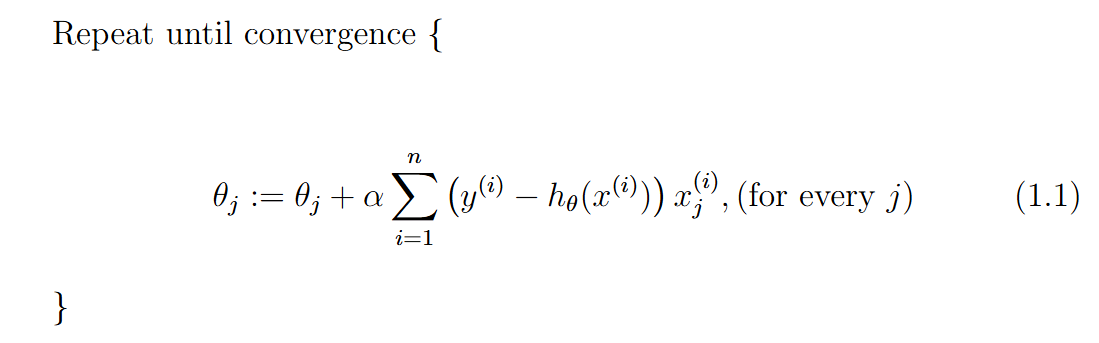
\includegraphics[width=0.8\textwidth]{images19.png} 
		\caption{batch gradient descent(批量梯度下降)}
	\end{figure}

  \begin{figure}[h]
		\centering 
		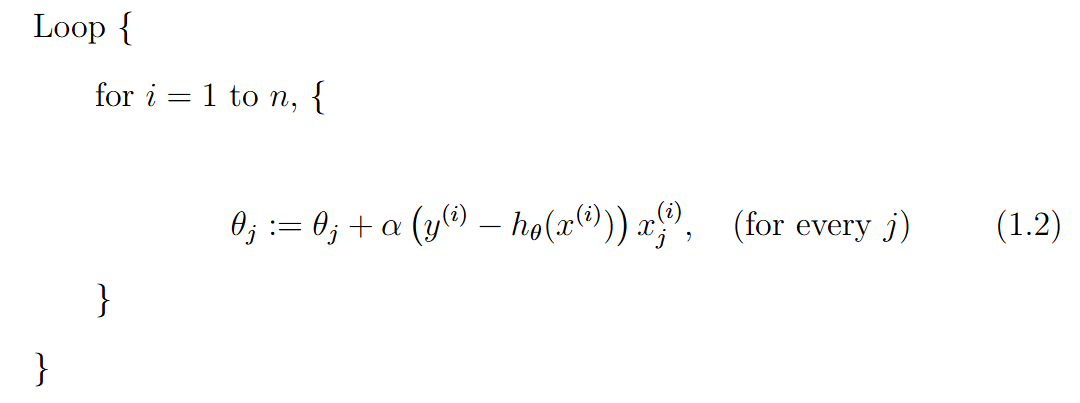
\includegraphics[width=0.8\textwidth]{images20.png} 
		\caption{stochastic gradient descent(随机梯度下降)}
	\end{figure}

\textbf{反思它们各自的优缺点:} batch gradient descent可以收敛到最优值,stochastic gradient descent计算量小.

\hspace*{\fill}

Matrix derivatives(矩阵导数)

  \begin{figure}[h]
		\centering 
		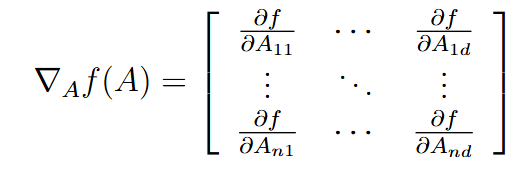
\includegraphics[width=0.55\textwidth]{images21.png} 
	\end{figure}

Least squares revisited(重新审视最小二乘法),考虑直接求解$\theta$的最优值.

  \begin{figure}[h]
		\centering 
		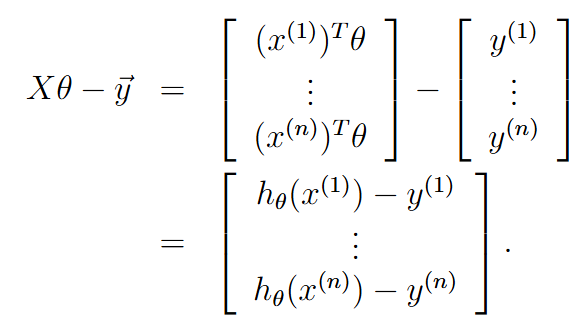
\includegraphics[width=0.55\textwidth]{images22.png} 
	\end{figure}

  \begin{figure}[h]
		\centering 
		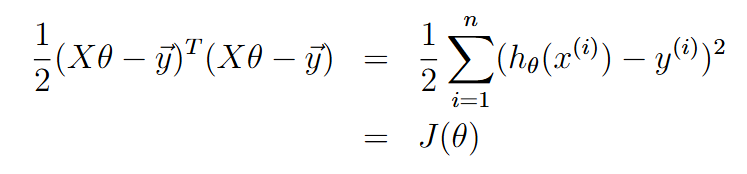
\includegraphics[width=0.65\textwidth]{images23.png} 
	\end{figure}

接下来我们对$J(\theta)$求导,对于矩阵求导我们有如下结论$\nabla_{x}b^{T}x=b$,$\nabla_{x}x^{T}Ax=Ax+A^{T}x$

\begin{equation}
\begin{aligned}
\nabla_{\theta}J(\theta) &= \nabla_{\theta}\dfrac{1}{2}(X\theta - \vec{y})^{T}(X\theta - \vec{y}) \\
   &= \dfrac{1}{2}\nabla_{\theta}(\theta^T(X^{T}X)\theta-2(X^T\vec{y})^{T}\theta) \\
   &= XX^T\theta-X^T\vec{y}
\end{aligned}
\end{equation}

如是我们得到\[\theta=(XX^T)^{-1}X^T\vec{y}\]也被称为normal equations.

\hspace*{\fill}

locally weighted linear regression (LWR) algorithm(局部参数线性回归):

  \begin{figure}[h]
		\centering 
		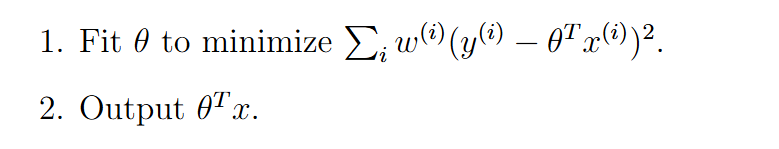
\includegraphics[width=0.65\textwidth]{images24.png} 
	\end{figure}


\section{Classification and logistic regression}

对于二分类问题,我们希望预测得到$y\in \{0,1\}$,上一章的Linear regression在这样的问题上表现不佳.因此我们对其进行改进,修改我们的假设函数$h_{\theta}(x)$\[h_{\theta}(x)=g(\theta^{T}x)=\dfrac{1}{1+e^{-\theta^{T}x}}\]其中\[g(z)=\dfrac{1}{1+e^{-z}}\]被称为logistic function或者sigmoid function.

  \begin{figure}[h]
		\centering 
		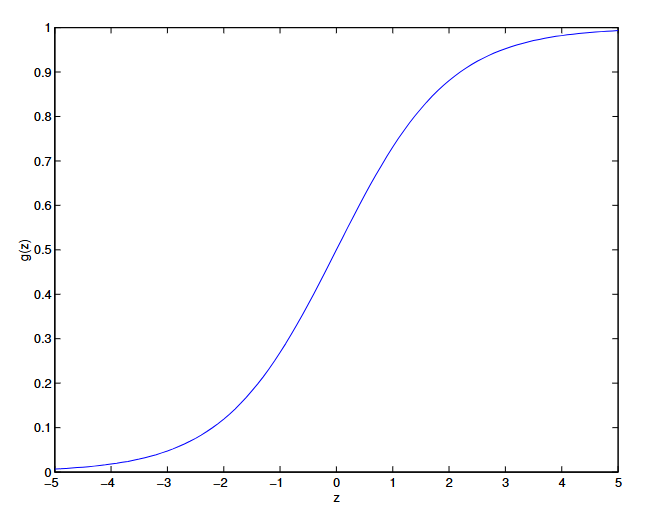
\includegraphics[width=0.55\textwidth]{images25.png} 
		\caption{sigmoid function}
	\end{figure}

如是我们假设\[P(y=1|x;\theta)=h_{\theta}(x)\] \[P(y=0|x;\theta)=1-h_{\theta}(x)\]整理可得\[p(y|x;\theta)=(h_{\theta}(x))^y(1-h_{\theta}(x))^{1-y}\]那么对于$n$个样本的情况\[L(\theta)=p(\vec{y}|X;\theta)=\prod_{i=1}^{n}(h_{\theta}(x^{(i)}))^{y^{(i)}}(1-h_{\theta}(x^{(i)}))^{1-y^{(i)}}\]对其最大化似然\[\ell(\theta)=\log {L(\theta)}=\sum_{i=1}^{n}y^{(i)}\log{h(x^{(i)})}+(1-y^{(i)})\log({1-h(x^{(i)})})\]

对其进行导数计算,注意到$g'(z)=g(z)(1-g(z))$

  \begin{figure}[h]
		\centering 
		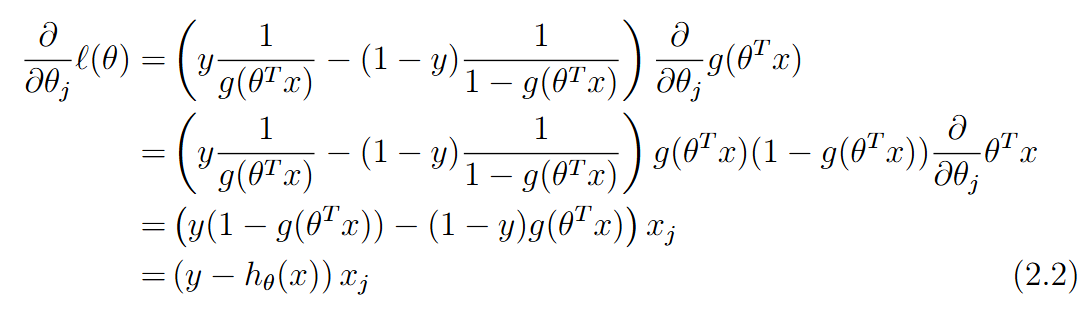
\includegraphics[width=0.85\textwidth]{images26.png} 
	\end{figure}

如是我们得到了随机梯度上升规则(stochastic gradient ascent rule)\[\theta_{j}:=\theta_{j}+\alpha (y^{(i)}-h_{\theta}(x^{(i)}))x_j^{(i)}\]

\textbf{Digression: the perceptron learning algorithm}

当我们修改$g(z)$的定义为

  \begin{figure}[ht]
		\centering 
		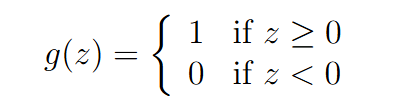
\includegraphics[width=0.35\textwidth]{images27.png} 
	\end{figure}

同时采用如上更新原则

  \begin{figure}[ht]
		\centering 
		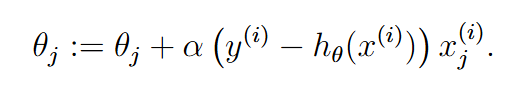
\includegraphics[width=0.5\textwidth]{images28.png} 
	\end{figure}

遂得到感知器学习算法(感知器学习算法).

\hspace*{\fill}

为了加快参数的收敛速度,我们下面了解Newton's method.我们可以用如下更新规则使得$f(\theta)=0$,\[\theta := \theta-\dfrac{f(\theta)}{f'(\theta)}\]令$f(\theta)=\ell '(\theta)$,我们得到最大化$\ell$的更新规则,\[\theta:=\theta-\dfrac{\ell '(\theta)}{\ell ''(\theta)}\]

Something to think about: How would this change if we wanted to use
Newton’s method to minimize rather than maximize a function?\[\theta:=\theta+\dfrac{\ell '(\theta)}{\ell ''(\theta)}\]

对于逻辑回归问题,需要修改更新规则,\[\theta:=\theta-H^{-1}\nabla_{\theta}\ell(\theta)\]其中\[H_{ij}=\dfrac{\partial ^2 \ell(\theta)}{\partial \theta_i \partial \theta_j}\]注意到在更新规则中存在矩阵求逆运算,故而虽然牛顿法的迭代速度很快,但是如果数据维数过高会导致单次迭代运算量极大.

\section{Generative learning algorithms}

\textbf{Generative learning algorithms:生成式学习算法}

尝试直接学习$p(y|x)$的算法(例如逻辑回归),或尝试直接学习从输入空间$\chi$到标签\{0,1\}的映射的算法(例如感知器算法)被称为判别性学习算法(discriminative learning algorithm),我们将要讨论尝试对$p(x|y)$和$p(y)$建模的算法,也被称为生成式学习算法(generative learning algorithms).

利用Bayes rule,\[p(y|x)=\dfrac{p(x|y)p(y)}{p(x)}\]

\hspace*{\fill}

\textbf{Gaussian discriminant analysis:高斯判别算法}

关于多元高斯分布,

  \begin{figure}[ht]
		\centering 
		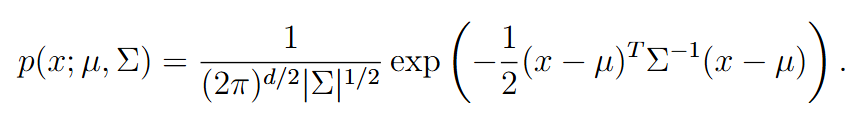
\includegraphics[width=0.9\textwidth]{images29.png} 
	\end{figure}

  \begin{figure}[ht]
		\centering 
		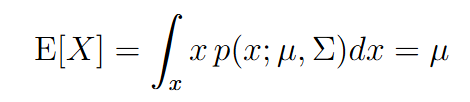
\includegraphics[width=0.45\textwidth]{images30.png} 
	\end{figure}

  \begin{figure}[ht]
		\centering 
		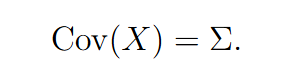
\includegraphics[width=0.3\textwidth]{images31.png} 
	\end{figure}

The Gaussian discriminant analysis model.该模型使用多元正态分布对 $p(x|y)$ 进行建模,具体如下images1,images2:

  \begin{figure}[h]
		\centering 
		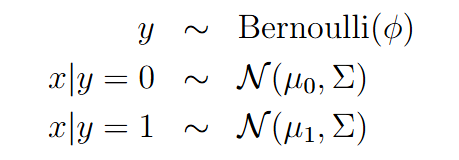
\includegraphics[width=0.5\textwidth]{images32.png} 
		\caption{images1}
	\end{figure}

  \begin{figure}[h]
		\centering 
		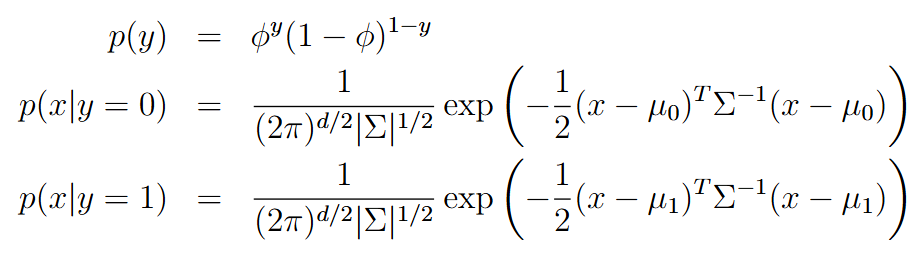
\includegraphics[width=0.85\textwidth]{images33.png} 
		\caption{images2}
	\end{figure}

得到如下似然函数,见images3

  \begin{figure}[h]
		\centering 
		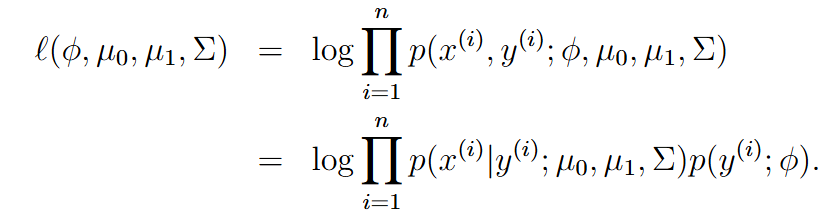
\includegraphics[width=0.85\textwidth]{images34.png} 
\caption{images3}
	\end{figure}

最大化似然函数后我们得到,如images4

  \begin{figure}[h]
		\centering 
		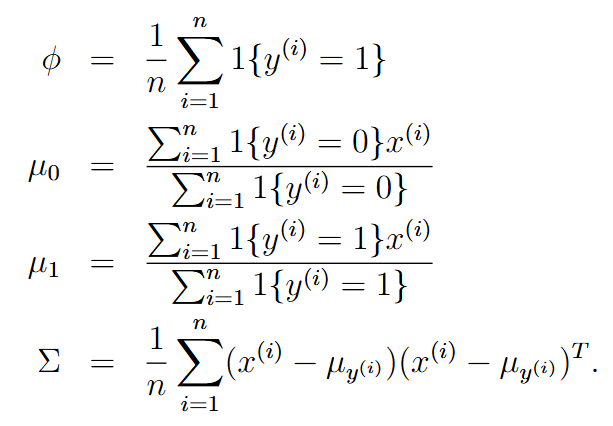
\includegraphics[width=0.6\textwidth]{images36.png} 
\caption{images4}
	\end{figure}

\hspace*{\fill}


\textbf{Discussion: GDA and logistic regression}

如果我们把$p(y=1|x;\phi,\mu_0,\mu_1,\Sigma)$看成一个关于$x$的函数,我们会发现\[p(y=1|x;\phi,\mu_0,\mu_1,\Sigma)=\dfrac{1}{1+exp(-\theta^{T}x)}\]其中$\theta$是$\phi,\mu_0,\mu_1,\Sigma$的某个适当函数.

\hspace*{\fill}

我们发现GDA和logistic regression具有某些联系.可以理解为,GDA在建模假设的过程中做出了更强的假设.这导致如果数据分布符合多维高斯分布,GDA的表现会优于logistic regression.由于做出明显较弱的假设,逻辑回归也更加稳健,并且对不正确的建模假设不太敏感.


\newpage


\section{Support vector machines}

\textbf{Support vector machines:支持向量机}

对SVM问题,我们修改原有的符号,$y\in \{-1,1\}$,同时将我们的分类器改写为\[h_{w,b}(x)=g(w^{T}x+b)\]

\textbf{Functional and geometric margins}

我们定义功能边距(functional margin)\[\hat{\gamma}^{(i)}=y^{(i)}(w^{T}x^{(i)}+b).\]可以发现当$w^{T}x^{(i)}+b$的值越来越大,我们对自己的正预测越具有信心,同理对反预测效果相同.考虑到对于$w,b$的自由缩放对$g(w^{T}x^{(i)}+b)$的影响,我们需要对其归一化,用$\dfrac{w}{||w||^2},\dfrac{b}{||w||^2}$对其替代.对于数据集$S=\{(x^{(i)},y^{(i)});i=1,...,n\}$,我们定义\[\hat{\gamma}=\min_{i=1,..,n}\hat{\gamma}^{(i)}\]

\hspace*{\fill}

\textbf{geometric margins}

我们定义几何边距(geometric margins)\[\gamma^{(i)}=y^{(i)}((\dfrac{w}{||w||})^{T}x^{(i)}+\dfrac{b}{||w||})\]那么同理\[{\gamma}=\min_{i=1,..,n}{\gamma}^{(i)}\]

\hspace*{\fill}

\textbf{The optimal margin classifier(最优间隔分类器)}

我们如何找到实现最大几何边距的那个超平面,可以将其转化为如下优化问题:

  \begin{figure}[h]
		\centering 
		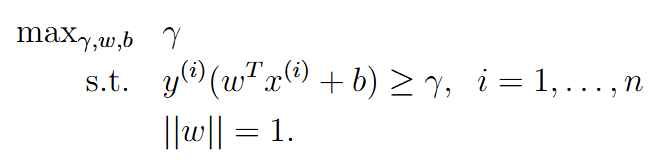
\includegraphics[width=0.8\textwidth]{images37.png} 
	\end{figure}

现在的问题是$"||w||=1"$是一个非常难处理的非凸约束.故而我们尝试修改问题形式:

  \begin{figure}[h]
		\centering 
		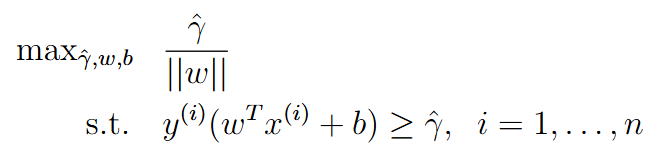
\includegraphics[width=0.8\textwidth]{images38.png} 
	\end{figure}

此时这个问题依旧不易处理,因为我们的目标$\dfrac{\hat{\gamma}}{||w||}$是非凸的.由于可以在$ w $和$ b $上添加任意缩放约束而不改变任何东西,故而我们令\[\hat{\gamma}=1.\]如是前面的优化问题等价于如下问题:

  \begin{figure}[h]
		\centering 
		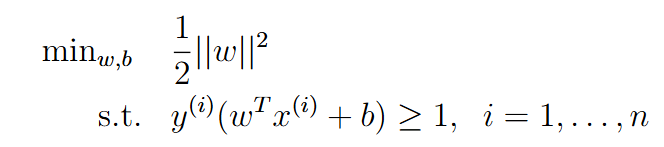
\includegraphics[width=0.8\textwidth]{images39.png} 
	\end{figure}

这是一个具有凸二次目标且仅具有线性约束的优化问题,我们可以解决它.

\hspace*{\fill}


\textbf{Lagrange duality(拉格朗日对偶性)}

考虑如下形式的问题:

  \begin{figure}[h]
		\centering 
		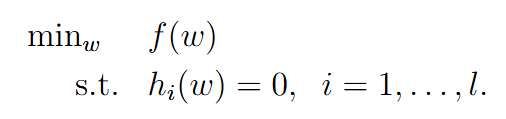
\includegraphics[width=0.5\textwidth]{images47.png} 
	\end{figure}

我们定义拉格朗日函数

\[\mathcal{L}(w,\beta)=f(w)+\sum_{i=1}^{l}\beta_i h_i(w)\]

我们定义原始优化问题

  \begin{figure}[h]
		\centering 
		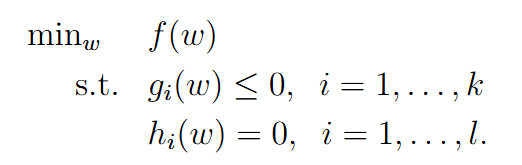
\includegraphics[width=0.5\textwidth]{images48.png} 
	\end{figure}

为了处理这种问题,我们定义广义拉格朗日函数\[\mathcal{L}(w,\alpha,\beta)=f(w)+\sum_{i=1}^{k}\alpha_i g_i(w)+ \sum_{i=1}^{l}\beta_i h_i(w)\]

Karush-Kuhn-Tucker (KKT) conditions

  \begin{figure}[h]
		\centering 
		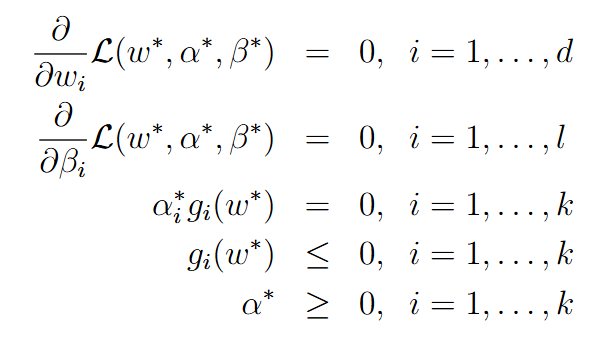
\includegraphics[width=0.5\textwidth]{images49.png} 
	\end{figure}


\textbf{SMO algorithm}

  \begin{figure}[h]
		\centering 
		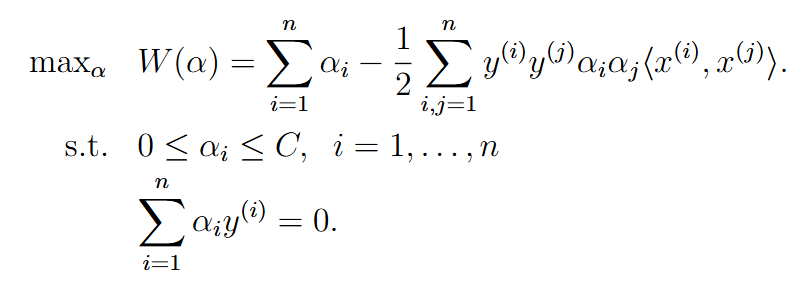
\includegraphics[width=0.8\textwidth]{images50.png} 
	\end{figure}

  \begin{figure}[h]
		\centering 
		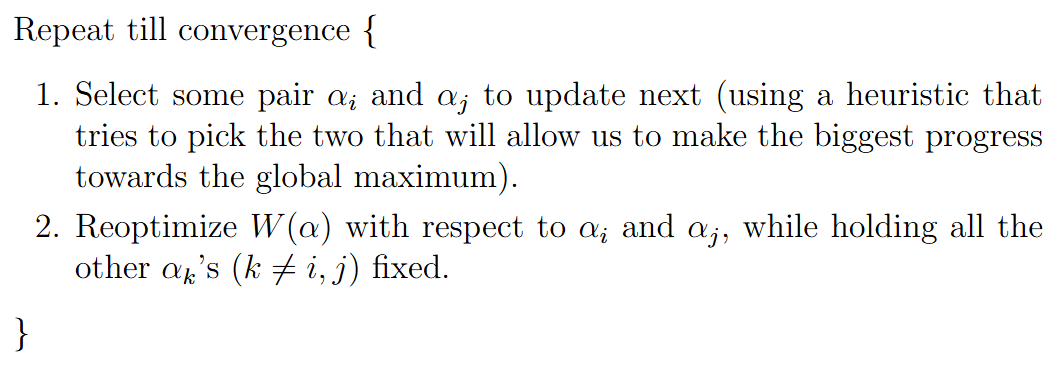
\includegraphics[width=0.9\textwidth]{images51.png} 
	\end{figure}


\section{Kernel methods}

\textbf{Kernel methods(内核方法)}

我们利用$\phi(x)$对输入特征进行升维,此时LMS的更新原则会随之改变为

  \begin{figure}[h]
		\centering 
		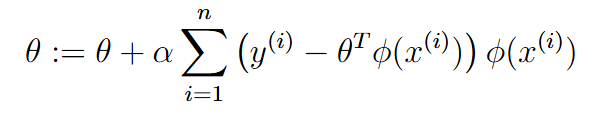
\includegraphics[width=0.5\textwidth]{images53.png} 
	\end{figure}

当维度变高时,参数更新的成本随之增加.所以我们需要找到一种不需要明确存储$\theta$的内核技巧.\[\theta=\sum_{i=1}^{n}\beta_i \phi(x^{(i)})\]如是更新原则变为

  \begin{figure}[h]
		\centering 
		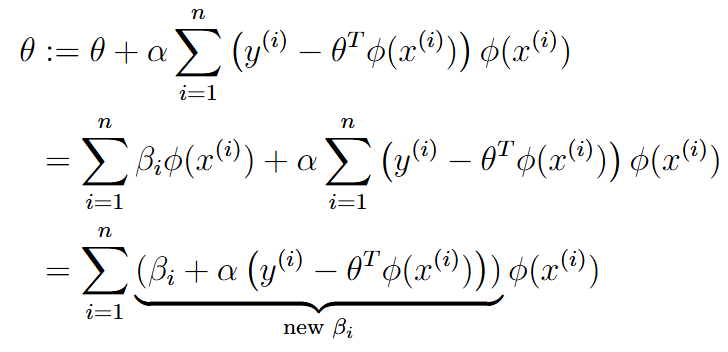
\includegraphics[width=0.75\textwidth]{images54.png} 
	\end{figure}

也即\[\beta_i:=\beta_i+\alpha(y^{(i)}-\theta^{T}\phi(x^{(i)}))\]

在替换掉$\theta$后

  \begin{figure}[h]
		\centering 
		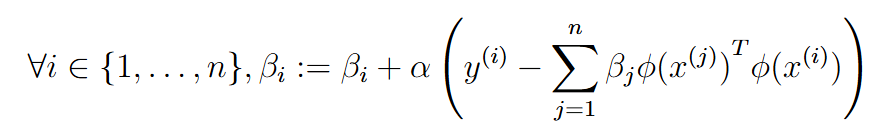
\includegraphics[width=0.75\textwidth]{images55.png} 
	\end{figure}

注意$\phi(x^{(j)})^{T}\phi(x^{(i)})$等同于$<\phi(x^{(j)}),\phi(x^{(i)})>$,由于它非常重要,我们有如下定义\[K(x,z)\triangleq <\phi(x),\phi(z)>\]如是最后的算法可以写成

  \begin{figure}[h]
		\centering 
		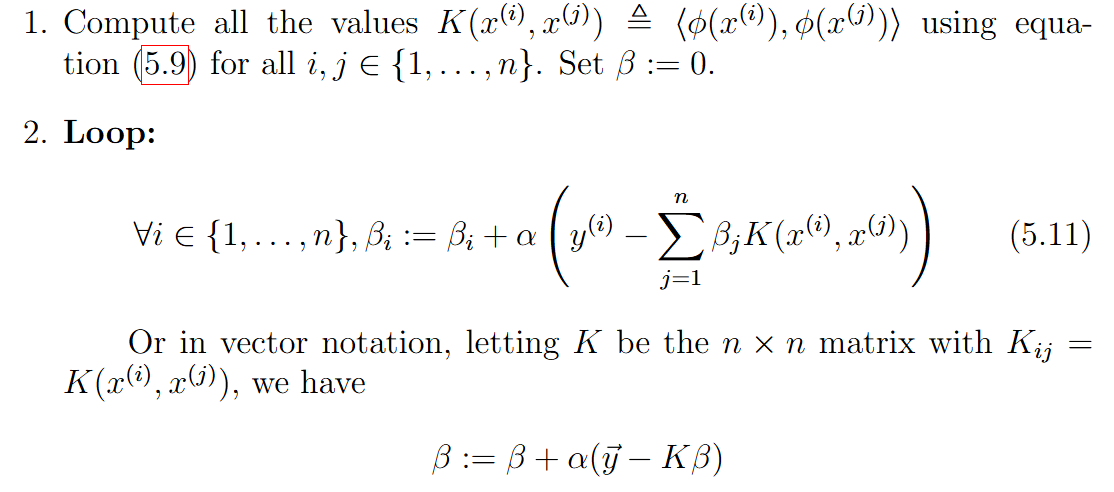
\includegraphics[width=0.95\textwidth]{images57.png} 
	\end{figure}

\newpage

\textbf{Application of kernel methods}

\hspace*{\fill}


\chapter{Foundations of Data Science}

\section{Reservoir Sampling}


















\chapter{CS106L}

\section{Types and Structs}

  \begin{figure}[h]
		\centering 
		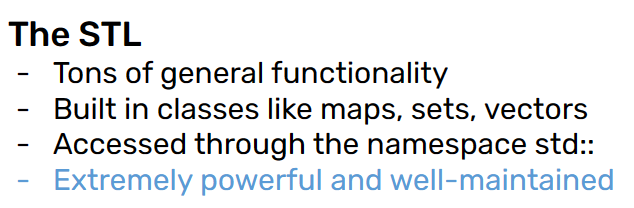
\includegraphics[width=0.7\textwidth]{images1.png} 
	\end{figure}

STL = Standard Template Library

\begin{lstlisting}[language=c++]
#include <string>
int val = 5; //32 bits (usually)
char ch = 'F'; //8 bits (usually)
float decimalVal1 = 5.0; //32 bits (usually)
double decimalVal2 = 5.0; //64 bits (usually)
bool bVal = true; //1 bit
std::string str = "Haven";
\end{lstlisting}

Fill in the blanks!

  \begin{figure}[h]
		\centering 
		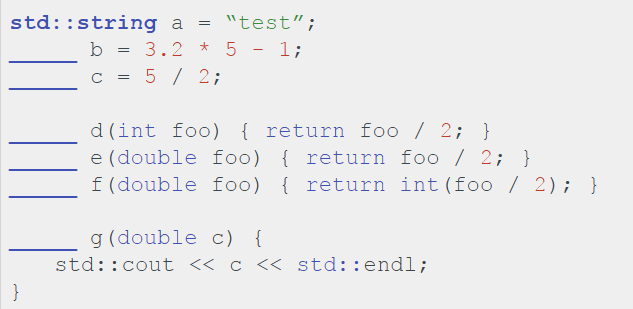
\includegraphics[width=0.7\textwidth]{images2.png} 
	\end{figure}

\subsection{Function overloading}

In C++, you cannot define multiple identical functions.But what if we want two versions of a function for two different types?---Function overloading.

Function Overloading = Define two functions with the same name but different types.

\begin{lstlisting}[language=c++]
int half(int x) {
    std::cout << “1” << endl; // (1)
    return x / 2;
}

double half(double x) {
    cout << “2” << endl; // (2)
    return x / 2;
}

half(3) // uses version (1), returns 1
half(3.0) // uses version (2), returns 1.5
\end{lstlisting}

The principle for selecting the function to call in C++ function overloading is as follows:

1.The compiler first looks for an exact match between the arguments passed in the function call and the parameters of each overloaded function. If an exact match is found, that function is selected.

2.If an exact match is not found, the compiler tries to find a function where the arguments can be implicitly converted to match the parameter types. This includes promotions, such as converting an int to a double.

3.If no exact match or promotion is found, the compiler considers standard conversions, such as integral promotions and conversions between arithmetic types.

4.If the previous steps do not yield a match, the compiler checks for user-defined conversions, such as invoking constructors or conversion operators.

5.If none of the above rules match, the compiler considers functions with ellipsis (...) parameters, which accept a variable number of arguments.

\begin{lstlisting}[language=c++]
int half(int x, int divisor = 2) { // (1)
    return x / divisor;
}

double half(double x) { // (2)
    return x / 2;
}

half(4)// uses version (1), returns 2
half(3, 3)// uses version (1), returns 1
half(3.0) // uses version (2), returns 1.5
\end{lstlisting}

\subsection{struct}

struct: a group of named
variables
each with their
own type. A way to
bundle different types
together


\begin{lstlisting}[language=c++]
struct Student {
    string name; // these are called fields
    string state; // separate these by semicolons
    int age;
};
Student s;
s.name = "Sarah";
s.state = "CA";
s.age = 21; // use . to access fields
\end{lstlisting}

Abbreviated Syntax to Initialize a struct.

\begin{lstlisting}[language=c++]
Student s;
s.name = "Sarah";
s.state = "CA";
s.age = 21;
//is the same as ...
Student s = {"Sarah", "CA", 21};
\end{lstlisting}

\subsection{std::pair}

std::pair: An STL
built-in struct with
two fields
of any type.

std::pair is a template: You specify the types of the
fields inside <> for each pair object you make.

The fields in std::pairs are named first and
second.

\begin{lstlisting}[language=c++]
std::pair<int, string> numSuffix = {1,"st"};
cout << numSuffix.first << numSuffix.second;
//prints 1st
\end{lstlisting}

\begin{lstlisting}[language=c++]
std::pair<bool, Student> lookupStudent(string name) {
    Student blank;
    if (notFound(name)) return std::make_pair(false, blank);
    Student result = getStudentWithName(name);
    return std::make_pair(true, result);
}
std::pair<bool, Student> output = lookupStudent(“Julie”);
\end{lstlisting}

\subsection{auto}

auto: Keyword used in
lieu of type when
declaring a variable, tells
the compiler to deduce
the type.

\begin{lstlisting}[language=c++]
// What types are these?
auto a = 3; // int
auto b = 4.3; // double
auto c = ‘X’; // char
auto d = “Hello”; // char* (a C string)
auto e = std::make_pair(3, “Hello”);
// std::pair<int, char*>
\end{lstlisting}

Keypoint:

- Everything with a name in your program has a type

- Static type system prevent errors before your code runs!

- Structs are a way to bundle a bunch of variables of many
types

- std::pair is a type of struct that had been defined for you
and is in the STL

- So you access it through the std:: namespace (std::pair)

- auto is a keyword that tells the compiler to deduce the
type of a variable, it should be used when the type is
obvious or very cumbersome to write out

\section{Initialization \& References}

Initialization: How we
provide initial
values to variables.

\begin{lstlisting}[language=c++]
Student s; // initialization after we declare
s.name = "Sarah";
s.state = "CA";
s.age = 21;
//is the same as ...
Student s = {"Sarah", "CA", 21};
// initialization while we declare
\end{lstlisting}

Multiple ways to initialize a pair.

\begin{lstlisting}[language=c++]
std::pair<int, string> numSuffix1 = {1,"st"};
std::pair<int, string> numSuffix2;
numSuffix2.first = 2;
numSuffix2.second = "nd";
std::pair<int, string> numSuffix2 = std::make_pair(3, "rd");
\end{lstlisting}

\subsection{Uniform initialization}

Uniform initialization: curly
bracket initialization. Available
for all types, immediate
initialization on declaration!

\begin{lstlisting}[language=c++]
std::vector<int> vec{1,3,5};
std::pair<int, string> numSuffix1{1,"st"};
Student s{"Sarah", "CA", 21};
// less common/nice for primitive types, but
possible!
int x{5};
string f{"Sarah"};
\end{lstlisting}

\subsection{Structured Binding}

Structured binding lets you initialize directly from
the contents of a struct.

\begin{lstlisting}[language=c++]
auto p =
std::make_pair(“s”, 5);
auto [a, b] = p;
// a is string, b is int
// auto [a, b] = std::make_pair(...);
\end{lstlisting}

Using Structured Binding.


\begin{lstlisting}[language=c++]
int main() {
    int a, b, c;
    std::cin >> a >> b >> c;
    auto [found, solutions] = quadratic(a, b, c);
    if (found) {
        auto [x1, x2] = solutions;
        std::cout << x1 << “ ” << x2 << endl;
    } else {
        std::cout << “No solutions found!” << endl;
        }
}
\end{lstlisting}

\subsection{Reference}

Reference: An alias
(another name) for a
named variable.

\begin{lstlisting}[language=c++]
void changeX(int& x){ // changes to x will persist
    x = 0;
}
void keepX(int x){
    x = 0;
}
int a = 100;
int b = 100;
changeX(a); // a becomes a reference to x
keepX(b); // b becomes a copy of x
cout << a << endl; //0
cout << b << endl; //100
\end{lstlisting}

\subsection{std::vector}

\begin{lstlisting}[language=c++]
std::vector<int> v;
std::vector<int> v(n, k);
v.push_back(k);
v[i] = k;
int k = v[i];
v.empty();
v.size();
v.clear();
// stay tuned
// stay tuned
\end{lstlisting}

“=” automatically makes
a copy! Must use \& to
avoid this.

\begin{lstlisting}[language=c++]
void shift(vector<std::pair<int, int>>& nums) {
    for (size_t i = 0; i < nums.size(); ++i) {
        auto& [num1, num2] = nums[i];
        num1++;
        num2++;
    }
}
\end{lstlisting}


\subsection{l-values vs r-values}

  \begin{figure}[ht]
		\centering 
		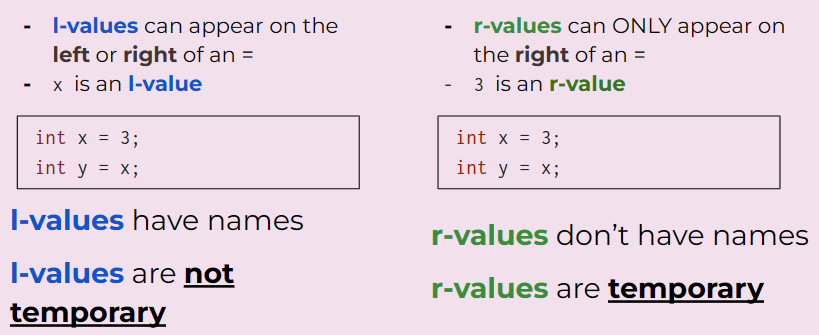
\includegraphics[width=0.8\textwidth]{images3.png} 
	\end{figure}


The classic reference-rvalue error.

\begin{lstlisting}[language=c++]
void shift(vector<std::pair<int, int>>& nums) {
    for (auto& [num1, num2]: nums) {
        num1++;
        num2++;
    }
}
shift({{1, 1}});
// {{1, 1}} is an rvalue, it can’t be referenced
\end{lstlisting}

\subsection{Const and Const References}

const indicates a variable can’t be modified!

\begin{lstlisting}[language=c++]
std::vector<int> vec{1, 2, 3};
const std::vector<int> c_vec{7, 8}; // a const variable
std::vector<int>& ref = vec; // a regular reference
const std::vector<int>& c_ref = vec; // a const reference
vec.push_back(3); // OKAY
c_vec.push_back(3); // BAD - const
ref.push_back(3); // OKAY
c_ref.push_back(3); // BAD - const
\end{lstlisting}

Can’t declare non-const reference to const variable!

\begin{lstlisting}[language=c++]
const std::vector<int> c_vec{7, 8}; // a const variable
// BAD - can't declare non-const ref to const vector
std::vector<int>& bad_ref = c_vec;
\end{lstlisting}

const \& subtleties

\begin{lstlisting}[language=c++]
std::vector<int> vec{1, 2, 3};
const std::vector<int> c_vec{7, 8};
std::vector<int>& ref = vec;
const std::vector<int>& c_ref = vec;
auto copy = c_ref; // a non-const copy
const auto copy = c_ref; // a const copy
auto& a_ref = ref; // a non-const reference
const auto& c_aref = ref; // a const reference
\end{lstlisting}

When do we use references/const references?

- If we’re working with a variable that takes up little
space in memory (e.g. int, double), we don’t need to
use a reference and can just copy the variable

- If we need to alias the variable to modify it, we can
use references

- If we don’t need to modify the variable, but it’s a big
variable (e.g. std::vector), we can use const references


\section{Streams}

stream: an abstraction for
input/output. Streams
convert between
data and
the string representation
of data.


\begin{lstlisting}[language=c++]
// use a stream to print any primitive type!
std::cout << 5 << std::endl; // prints 5
// and most from the STL work!
std::cout << "Sarah" << std::endl;
// Mix types!
std::cout << "Sarah is " << 21 << std::endl;
// structs?
Student s = {"Sarah", "CA", 21};
std::cout << s << std::endl; //ERROR!
std::cout << s.name << s.age << std::endl;
\end{lstlisting}

std::cout is an
output
stream. It has type
std::ostream.

  \begin{figure}[h]
		\centering 
		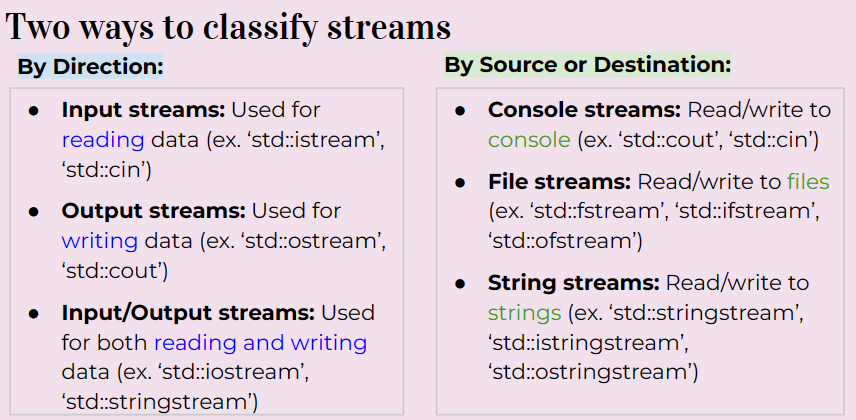
\includegraphics[width=1.0\textwidth]{images4.png} 
	\end{figure}


\subsection{Output Streams}

- Have type std::ostream

- You can only send data to the stream

- Interact with the stream using the << operator

- Converts any type into string and sends it to the
stream

- std::cout is the output stream that goes to the console

\begin{lstlisting}[language=c++]
std::cout << 5 << std::endl;
// converts int value 5 to string “5”
// sends “5” to the console output stream
\end{lstlisting}


\subsection{Output File Streams}

- Have type std::ofstream

- You can only send data to file using the << operator

- Converts data of any type into a string and sends it
to the file stream

- Must initialize your own ofstream object linked to your
file

\begin{lstlisting}[language=c++]
std::ofstream out(“out.txt”);
// out is now an ofstream that outputs to
out.txt
out << 5 << std::endl; // out.txt contains 5
\end{lstlisting}

\subsection{Input Streams}

- Have type std::istream

- You can only receive strings using the >> operator

- Receives a string from the stream and converts it to
data

- std::cin is the input stream that gets input from the
console

\begin{lstlisting}[language=c++]
int x;
string str;
std::cin >> x >> str;
//reads exactly one int then one string from
console
\end{lstlisting}

Nitty Gritty Details: std::cin

- First call to std::cin >> creates a command line
prompt that allows the user to type until they hit enter

- Each >> ONLY reads until the next whitespace

- Whitespace = tab, space, newline

- Everything after the first whitespace gets saved and
used the next time std::cin >> is called

- The place its saved is called a buffer!

- If there is nothing waiting in the buffer, std::cin >>
creates a new command line prompt

- Whitespace is eaten; it won’t show up in output


\subsection{Stringstreams}

\begin{lstlisting}[language=c++]
std::string input = "123";
std::stringstream stream(input);
int number;
stream >> number;
std::cout << number << std::endl; // Outputs "123"
\end{lstlisting}


\section{Containers}

Container: An object that allows us to
collect other objects together and interact
with them in some way.





\chapter{Large Language Models for Personalized}



\chapter{Leetcode}

面对保研以及考研复试等中的机试,我们需要对常见算法题解法进行总结,如下内容默认解题使用cpp语言.

\section{基础知识}


\section{回溯法}

























\end{document}





